% =====================================================================
%  GloVe: the theory --- slide deck (no implementation details)
%  Build:  latexmk -pdf glove_theory_slides.tex
% =====================================================================
\documentclass[aspectratio=169,11pt]{beamer}

\usetheme[progressbar=frametitle,numbering=fraction,block=fill]{metropolis}
\usepackage[T1]{fontenc}
\usepackage{lmodern}
\usepackage{amsmath,amssymb,mathtools}
\usepackage{booktabs}
\usepackage{tikz}
\usetikzlibrary{arrows.meta,positioning,shapes.geometric,calc,decorations.pathreplacing,angles,quotes}
\usepackage{pgfplots}
\pgfplotsset{compat=1.18}

\definecolor{ink}{HTML}{1F2328}
\definecolor{accent}{HTML}{0969DA}
\definecolor{warn}{HTML}{CF222E}
\definecolor{okc}{HTML}{1A7F37}
\definecolor{stageA}{HTML}{DDF4FF}
\definecolor{stageB}{HTML}{FFF8C5}
\definecolor{stageC}{HTML}{FBEFFF}
\definecolor{stageD}{HTML}{DAFBE1}
\definecolor{wA}{HTML}{4C8BF5}
\definecolor{wB}{HTML}{F5A524}
\definecolor{wC}{HTML}{2DA44E}
\definecolor{wD}{HTML}{CF222E}
\definecolor{wE}{HTML}{8250DF}

\setbeamercolor{frametitle}{bg=ink}
\setbeamercolor{progress bar}{fg=accent}
\setbeamercolor{alerted text}{fg=warn}

\newcommand{\wv}{\mathbf{w}}
\newcommand{\cv}{\tilde{\mathbf{w}}}
\DeclareMathOperator{\PMI}{PMI}

\tikzset{
  arr/.style={-{Stealth[length=2.2mm]},thick},
  pt/.style={circle,fill,inner sep=1.6pt},
  box/.style={draw,rounded corners,align=center,font=\small},
  tok/.style={draw,rounded corners=2pt,minimum height=7mm,minimum width=10mm,font=\small,fill=white},
}

\title{GloVe: The Theory}
\subtitle{Why ratios of co-occurrence probabilities lead to a log-bilinear model}
\author{Global Vectors for Word Representation --- Pennington, Socher \& Manning (2014)}
\date{\today}

\begin{document}

\maketitle

\begin{frame}{Roadmap}
\begin{columns}[T]
\column{0.48\textwidth}
\begin{enumerate}
  \item Representing meaning with vectors
  \item Co-occurrence statistics
  \item Deriving the GloVe (Global Vectors) model
  \item The weighted objective
\end{enumerate}
\column{0.48\textwidth}
\begin{enumerate}\setcounter{enumi}{4}
  \item Connections: pointwise mutual information (PMI), singular value decomposition (SVD), skip-gram
  \item Complexity
  \item Empirical behaviour \& limitations
\end{enumerate}
\end{columns}
\end{frame}

\begin{frame}{Abbreviations used in this deck}
\small
\centering
\begin{tabular}{@{}ll@{\hspace{10mm}}ll@{}}
\toprule
AdaGrad & Adaptive gradient (optimiser)          & nnz   & Number of non-zero entries\\
BERT    & Bidirectional Encoder Representations  & PMI   & Pointwise mutual information\\
        & \quad from Transformers                & PPMI  & Positive PMI (negatives set to 0)\\
ELMo    & Embeddings from Language Models        & SG    & Skip-gram (word2vec model)\\
GloVe   & Global Vectors for Word Representation & SVD   & Singular value decomposition\\
LSA     & Latent Semantic Analysis               &       & \\
\bottomrule
\end{tabular}

\vspace{3mm}
\scriptsize Venue abbreviations (EMNLP, NeurIPS, JMLR, JASIS) are spelled out in the References.
\end{frame}

% =====================================================================
\section{Representing meaning}
% =====================================================================

\begin{frame}{The distributional hypothesis}
\begin{columns}[c]
\column{0.5\textwidth}
\begin{quote}
\emph{``You shall know a word by the company it keeps.''}\\ \hfill --- J.\,R.~Firth, 1957
\end{quote}
\begin{itemize}
  \item Words used in similar contexts tend to have similar meanings.
  \item So a word's meaning can be estimated from \alert{statistics of the words around it}.
  \item Every embedding method --- Latent Semantic Analysis (LSA), word2vec, GloVe --- builds on this idea.
\end{itemize}
\column{0.5\textwidth}
\centering
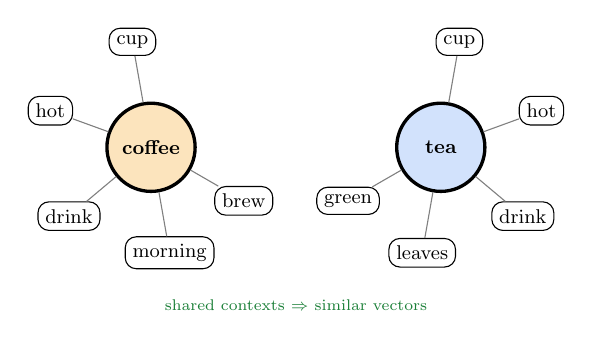
\begin{tikzpicture}[font=\small,scale=0.8,transform shape]
  \node[circle,draw,very thick,fill=wB!30,minimum size=14mm] (c) at (0,0) {\textbf{coffee}};
  \node[circle,draw,very thick,fill=wA!25,minimum size=14mm] (t) at (4.6,0) {\textbf{tea}};
  \foreach \w/\a in {cup/100,hot/160,drink/220,morning/280,brew/330}
     \node[box,fill=white] (x\w) at ($(c)+(\a:1.7)$) {\w};
  \foreach \w/\a in {cup/80,hot/20,drink/320,leaves/260,green/210}
     \node[box,fill=white] (y\w) at ($(t)+(\a:1.7)$) {\w};
  \foreach \w in {cup,hot,drink,morning,brew} \draw[gray] (c) -- (x\w);
  \foreach \w in {cup,hot,drink,leaves,green} \draw[gray] (t) -- (y\w);
  \node[font=\scriptsize,okc,align=center] at (2.3,-2.5) {shared contexts $\Rightarrow$ similar vectors};
\end{tikzpicture}
\end{columns}
\end{frame}

\begin{frame}{From symbols to geometry}
\begin{columns}[c]
\column{0.5\textwidth}
\centering
\textbf{One-hot} ($\mathbb R^{V}$, sparse)\\[2mm]
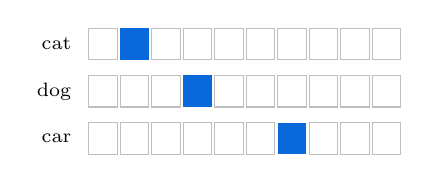
\begin{tikzpicture}[font=\scriptsize]
  \foreach \w/\k [count=\r from 0] in {cat/1,dog/3,car/6} {
    \node[anchor=east] at (-0.1,-\r*0.6) {\w};
    \foreach \j in {0,...,9} {
      \ifnum\j=\k \fill[accent] (\j*0.4,-\r*0.6-0.2) rectangle ++(0.36,0.4);
      \else \draw[gray!50] (\j*0.4,-\r*0.6-0.2) rectangle ++(0.36,0.4); \fi}}
\end{tikzpicture}

\vspace{2mm}
\small all pairs orthogonal: $\;\cos(\text{cat},\text{dog})=\cos(\text{cat},\text{car})=0$
\column{0.5\textwidth}
\centering
\textbf{Dense embedding} ($\mathbb R^{d}$, $d\ll V$)\\[2mm]
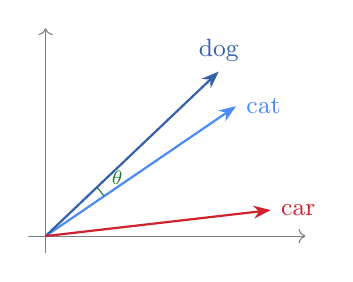
\begin{tikzpicture}[scale=1.1]
  \draw[->,gray] (-0.2,0) -- (3,0); \draw[->,gray] (0,-0.2) -- (0,2.4);
  \draw[arr,wA] (0,0) -- (2.2,1.5) node[right,font=\small]{cat};
  \draw[arr,wA!70!black] (0,0) -- (2.0,1.9) node[above,font=\small]{dog};
  \draw[arr,wD] (0,0) -- (2.6,0.3) node[right,font=\small]{car};
  \coordinate (o) at (0,0); \coordinate (c1) at (2.2,1.5); \coordinate (c2) at (2.0,1.9);
  \pic[draw,okc,"$\theta$",angle radius=9mm,angle eccentricity=1.3,font=\scriptsize] {angle=c1--o--c2};
\end{tikzpicture}

\vspace{1mm}
\small similarity $=\cos\theta=\dfrac{\wv_a^\top\wv_b}{\|\wv_a\|\|\wv_b\|}$
\end{columns}
\end{frame}

\begin{frame}{The goal: linear structure}
\begin{columns}[c]
\column{0.45\textwidth}
Good embeddings encode relations as \alert{consistent directions}:
\[\wv_{\text{king}}-\wv_{\text{man}}+\wv_{\text{woman}}\approx\wv_{\text{queen}}\]
\[\wv_{\text{Paris}}-\wv_{\text{France}}+\wv_{\text{Italy}}\approx\wv_{\text{Rome}}\]
\small
This is a \emph{design target}. The question GloVe asks is:\\
\emph{what model of the statistics makes such directions appear?}
\column{0.55\textwidth}
\centering
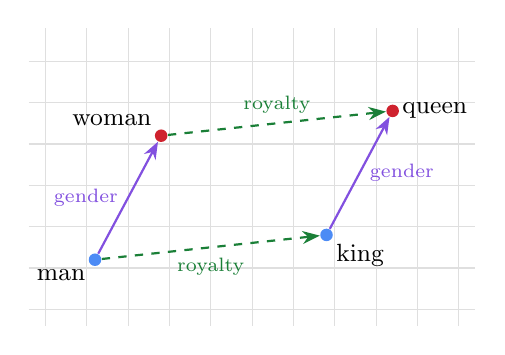
\begin{tikzpicture}[scale=1.05,lbl/.style={font=\small}]
  \draw[gray!25,step=0.5] (-0.2,-0.2) grid (5.2,3.4);
  \node[pt,wA] (man) at (0.6,0.6) {}; \node[lbl,below left] at (man) {man};
  \node[pt,wD] (woman) at (1.4,2.1) {}; \node[lbl,above left] at (woman) {woman};
  \node[pt,wA] (king) at (3.4,0.9) {}; \node[lbl,below right] at (king) {king};
  \node[pt,wD] (queen) at (4.2,2.4) {}; \node[lbl,right] at (queen) {queen};
  \draw[arr,wE] (man) -- node[left,font=\scriptsize]{gender} (woman);
  \draw[arr,wE] (king) -- node[right,font=\scriptsize]{gender} (queen);
  \draw[arr,okc,dashed] (man) -- node[below,font=\scriptsize]{royalty} (king);
  \draw[arr,okc,dashed] (woman) -- node[above,font=\scriptsize]{royalty} (queen);
\end{tikzpicture}
\end{columns}
\end{frame}

% =====================================================================
\section{Co-occurrence statistics}
% =====================================================================

\begin{frame}{The co-occurrence matrix $X$}
\begin{columns}[c]
\column{0.5\textwidth}
\centering
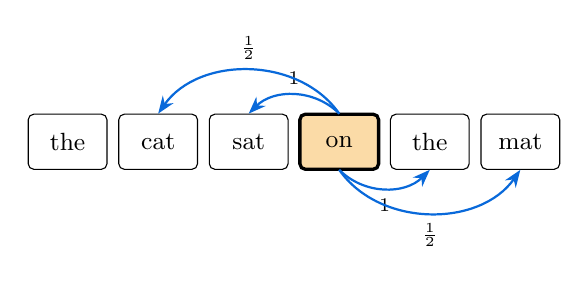
\begin{tikzpicture}
  \foreach \w [count=\k from 0] in {the,cat,sat,on,the,mat}
     \node[tok] (n\k) at (\k*1.15,0) {\w};
  \node[tok,fill=wB!40,very thick] at (n3) {on};
  \draw[arr,accent] (n3.north) to[bend right=45] node[above,font=\scriptsize,black]{1} (n2.north);
  \draw[arr,accent] (n3.north) to[bend right=55] node[above,font=\scriptsize,black]{$\frac12$} (n1.north);
  \draw[arr,accent] (n3.south) to[bend right=45] node[below,font=\scriptsize,black]{1} (n4.south);
  \draw[arr,accent] (n3.south) to[bend right=55] node[below,font=\scriptsize,black]{$\frac12$} (n5.south);
\end{tikzpicture}

\vspace{3mm}
\small
$X_{ij}$ = how often $j$ appears within a window around $i$.
Closer words count more (weight $1/\text{distance}$).
\column{0.5\textwidth}
\centering
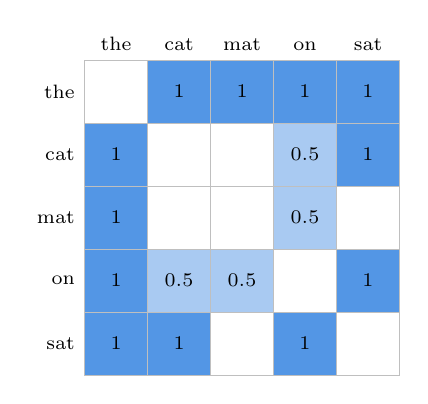
\begin{tikzpicture}
  \def\names{the,cat,mat,on,sat}
  \foreach \r [count=\i from 0] in {{0,1,1,1,1},{1,0,0,0.5,1},{1,0,0,0.5,0},{1,0.5,0.5,0,1},{1,1,0,1,0}} {
    \foreach \v [count=\j from 0] in \r {
      \pgfmathsetmacro{\pc}{\v*70}
      \node[draw=gray!50,minimum size=8mm,fill=accent!\pc,font=\scriptsize] at (\j*0.8,-\i*0.8)
         {\ifdim\v pt>0pt $\v$\fi};}}
  \foreach \n [count=\j from 0] in \names {
    \node[font=\scriptsize,above] at (\j*0.8,0.4) {\n};
    \node[font=\scriptsize,left] at (-0.4,-\j*0.8) {\n};}
\end{tikzpicture}

\small symmetric, mostly zeros, and \alert{global}: it summarises the whole corpus
\end{columns}
\end{frame}

\begin{frame}{Counts are heavy-tailed (Zipf)}
\begin{columns}[c]
\column{0.5\textwidth}
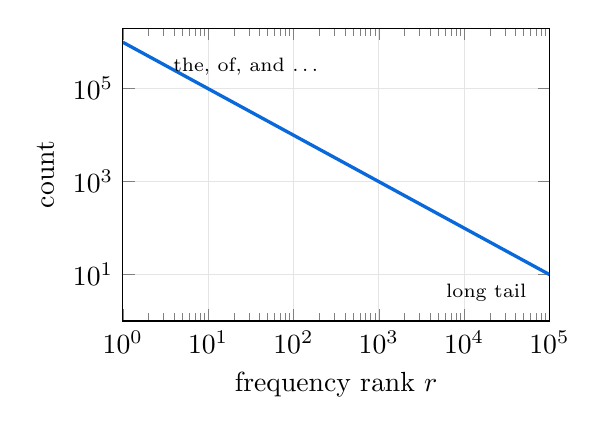
\begin{tikzpicture}
\begin{axis}[width=7cm,height=5.3cm,xmode=log,ymode=log,
  xlabel={frequency rank $r$},ylabel={count},grid=major,grid style={gray!20},
  xmin=1,xmax=1e5,ymin=1,ymax=2e6]
  \addplot[very thick,accent,domain=1:1e5,samples=60]{1e6/x};
  \node[font=\scriptsize,anchor=west] at (axis cs:3,3e5) {the, of, and \ldots};
  \node[font=\scriptsize,anchor=east] at (axis cs:7e4,4) {long tail};
\end{axis}
\end{tikzpicture}
\column{0.5\textwidth}\small
\begin{itemize}
  \item Word frequency $\propto 1/\text{rank}$, so a handful of words dominate.
  \item Co-occurrence counts are also heavy-tailed: a few huge cells and many cells equal to 1.
  \item Consequences for any model:
    \begin{itemize}\small
      \item raw counts are dominated by stop words;
      \item small counts are \alert{noisy};
      \item $\log X$ compresses the range, but $\log 0=-\infty$.
    \end{itemize}
\end{itemize}
\end{columns}
\end{frame}

\begin{frame}{From counts to probabilities}
\[
X_i=\sum_k X_{ik},\qquad P_{ik}=P(k\mid i)=\frac{X_{ik}}{X_i}
\]
\begin{columns}[c]
\column{0.5\textwidth}
\centering
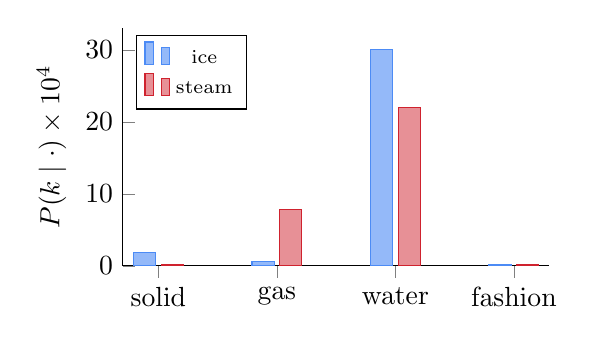
\begin{tikzpicture}
\begin{axis}[width=7cm,height=4.6cm,ybar,bar width=8pt,ymin=0,
  symbolic x coords={solid,gas,water,fashion},xtick=data,
  ylabel={$P(k\mid\cdot)\times10^{4}$},legend style={font=\scriptsize,at={(0.03,0.97)},anchor=north west},
  axis lines*=left]
  \addplot[fill=wA!60,draw=wA] coordinates {(solid,1.9) (gas,0.66) (water,30) (fashion,0.17)};
  \addplot[fill=wD!50,draw=wD] coordinates {(solid,0.22) (gas,7.8) (water,22) (fashion,0.18)};
  \legend{ice,steam}
\end{axis}
\end{tikzpicture}
\column{0.5\textwidth}\small
\begin{itemize}
  \item Raw conditional probabilities are hard to compare: ``water'' is large for \emph{both} words.
  \item What tells us about meaning is how the two distributions \alert{differ}.
\end{itemize}
{\scriptsize Values from Pennington et al.\ (2014), Table 1.}
\end{columns}
\end{frame}

\begin{frame}{The key insight: ratios}
\begin{columns}[c]
\column{0.45\textwidth}
\[
\frac{P_{ik}}{P_{jk}}=\frac{P(k\mid\text{ice})}{P(k\mid\text{steam})}
\]
\small
\begin{tabular}{lcl}
\toprule
$k$ & ratio & meaning\\
\midrule
solid & 8.9 & $k$ relates to ice\\
gas & 0.085 & $k$ relates to steam\\
water & 1.36 & relates to both\\
fashion & 0.96 & relates to neither\\
\bottomrule
\end{tabular}

\vspace{2mm}
Ratios cancel out the probe word's own frequency and keep only what \alert{discriminates} $i$ from $j$.
\column{0.55\textwidth}
\centering
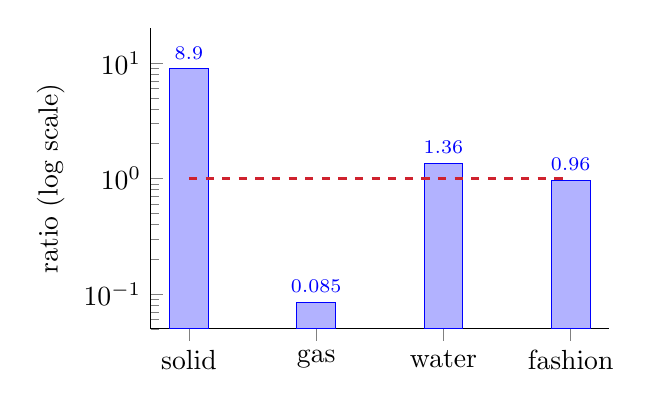
\begin{tikzpicture}
\begin{axis}[width=7.4cm,height=5.4cm,ybar,ymode=log,log origin=infty,
  ymin=0.05,ymax=20,bar width=14pt,
  symbolic x coords={solid,gas,water,fashion},xtick=data,
  ylabel={ratio (log scale)},axis lines*=left,
  point meta=rawy,nodes near coords,nodes near coords style={font=\scriptsize,/pgf/number format/.cd,fixed,precision=3},
  every axis plot/.append style={fill=accent!60,draw=accent}]
  \addplot coordinates {(solid,8.9) (gas,0.085) (water,1.36) (fashion,0.96)};
  \draw[dashed,warn,thick] (axis cs:solid,1) -- (axis cs:fashion,1);
\end{axis}
\end{tikzpicture}
\end{columns}
\end{frame}

% =====================================================================
\section{Deriving the model}
% =====================================================================

\begin{frame}{What we want}
Find vectors and a function $F$ such that
\[
\boxed{\;F(\wv_i,\wv_j,\cv_k)=\frac{P_{ik}}{P_{jk}}\;}
\]
\begin{itemize}
  \item $\wv_i,\wv_j\in\mathbb R^d$ are \emph{word} vectors; $\cv_k$ is a separate \emph{context} vector.
  \item The right-hand side is measured from the corpus; the left-hand side is the model.
  \item $F$ could be anything at this point. We now add \alert{three natural constraints} that pin it down.
\end{itemize}
\vfill
\centering
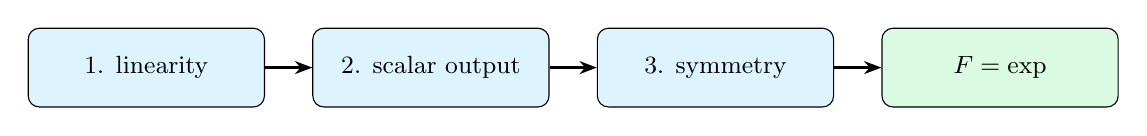
\begin{tikzpicture}[font=\small,node distance=6mm]
  \node[box,fill=stageA,minimum width=30mm,minimum height=10mm] (a) {1. linearity};
  \node[box,fill=stageA,minimum width=30mm,minimum height=10mm,right=of a] (b) {2. scalar output};
  \node[box,fill=stageA,minimum width=30mm,minimum height=10mm,right=of b] (c) {3. symmetry};
  \node[box,fill=stageD,minimum width=30mm,minimum height=10mm,right=of c] (d) {$F=\exp$};
  \draw[arr] (a)--(b); \draw[arr] (b)--(c); \draw[arr] (c)--(d);
\end{tikzpicture}
\end{frame}

\begin{frame}{Constraints 1 \& 2: differences and dot products}
\begin{columns}[c]
\column{0.5\textwidth}
\textbf{Linearity.} Vector spaces are linear, so compare $i$ and $j$ through their difference:
\[F(\wv_i-\wv_j,\ \cv_k)\]
\textbf{Scalar output.} The target is a scalar but the arguments are vectors. Use a dot product so that dimensions do not mix in arbitrary ways:
\[F\big((\wv_i-\wv_j)^{\top}\cv_k\big)=\frac{P_{ik}}{P_{jk}}\]
\column{0.5\textwidth}
\centering
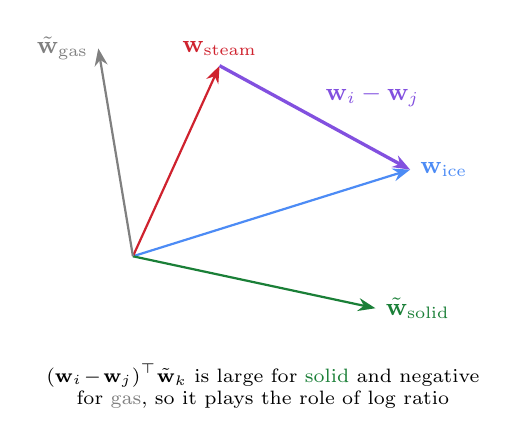
\begin{tikzpicture}[scale=1.1]
  \coordinate (o) at (0,0);
  \coordinate (wi) at (3.2,1.0); \coordinate (wj) at (1.0,2.2);
  \draw[arr,wA] (o) -- (wi) node[right,font=\small]{$\wv_{\text{ice}}$};
  \draw[arr,wD] (o) -- (wj) node[above,font=\small]{$\wv_{\text{steam}}$};
  \draw[arr,wE,very thick] (wj) -- (wi) node[midway,above right,font=\small]{$\wv_i-\wv_j$};
  \draw[arr,okc] (o) -- (2.8,-0.6) node[right,font=\small]{$\cv_{\text{solid}}$};
  \draw[arr,gray] (o) -- (-0.4,2.4) node[left,font=\small]{$\cv_{\text{gas}}$};
  \node[font=\scriptsize,align=center,text width=55mm] at (1.5,-1.5)
   {$(\wv_i-\wv_j)^\top\cv_k$ is large for \textcolor{okc}{solid} and negative for \textcolor{gray}{gas}, so it plays the role of $\log$ ratio};
\end{tikzpicture}
\end{columns}
\end{frame}

\begin{frame}{Constraint 3: symmetry forces $F=\exp$}
\small
The roles of word and context are arbitrary: swapping $\wv\leftrightarrow\cv$ and $X\leftrightarrow X^\top$ should leave the model unchanged.
Require $F$ to be a \alert{homomorphism} from $(\mathbb R,+)$ to $(\mathbb R_{>0},\times)$:
\[
F\big((\wv_i-\wv_j)^\top\cv_k\big)=\frac{F(\wv_i^\top\cv_k)}{F(\wv_j^\top\cv_k)}
\quad\Longrightarrow\quad F=\exp
\]
\begin{columns}[c]
\column{0.5\textwidth}
Matching numerator to numerator:
\[
\exp(\wv_i^\top\cv_k)=P_{ik}=\frac{X_{ik}}{X_i}
\]
\[
\wv_i^\top\cv_k=\log X_{ik}-\log X_i
\]
\column{0.5\textwidth}
\centering
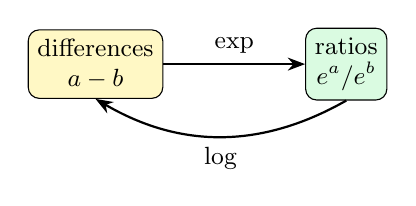
\begin{tikzpicture}[font=\small]
  \node[box,fill=stageB] (add) {differences\\$a-b$};
  \node[box,fill=stageD,right=18mm of add] (mul) {ratios\\$e^a/e^b$};
  \draw[arr] (add) -- node[above]{$\exp$} (mul);
  \draw[arr] (mul.south) to[bend left=30] node[below]{$\log$} (add.south);
\end{tikzpicture}
\end{columns}
\end{frame}

\begin{frame}{Restoring symmetry with biases}
\small
\begin{columns}[c]
\column{0.55\textwidth}
$\log X_i$ does not depend on $k$: absorb it into a bias $b_i$, and add $\tilde b_k$ for symmetry:
\[
\boxed{\;\wv_i^\top\cv_k+b_i+\tilde b_k=\log X_{ik}\;}
\]
\begin{itemize}\footnotesize
  \item A \alert{log-bilinear} model: bilinear in $(\wv,\cv)$ and linear in $\log X$.
  \item The biases absorb word frequency, so the vectors are free to encode \emph{relations}.
  \item Vector differences now reproduce log ratios:
  \[(\wv_i-\wv_j)^\top\cv_k=\log\tfrac{P_{ik}}{P_{jk}}+\text{const}\]
\end{itemize}
\column{0.45\textwidth}
\centering
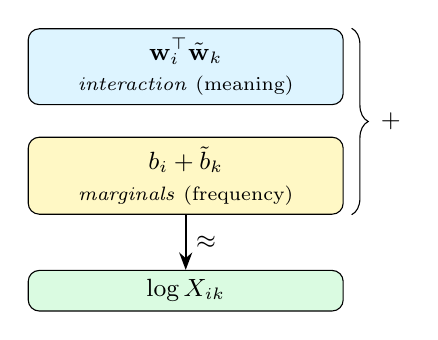
\begin{tikzpicture}[font=\small]
  \node[box,fill=stageA,minimum width=40mm] (m) {$\wv_i^\top\cv_k$\\ \scriptsize \emph{interaction} (meaning)};
  \node[box,fill=stageB,minimum width=40mm,below=4mm of m] (b) {$b_i+\tilde b_k$\\ \scriptsize \emph{marginals} (frequency)};
  \node[box,fill=stageD,minimum width=40mm,below=7mm of b] (x) {$\log X_{ik}$};
  \draw[decorate,decoration={brace,amplitude=6pt}] ($(m.north east)+(1mm,0)$) -- ($(b.south east)+(1mm,0)$) node[midway,right=7pt]{$+$};
  \draw[arr] (b) -- node[right]{$\approx$} (x);
\end{tikzpicture}
\end{columns}
\end{frame}

% =====================================================================
\section{The weighted objective}
% =====================================================================

\begin{frame}{Fitting it: why \emph{weighted} least squares?}
The equation cannot hold exactly, so fit it by regression. Unweighted least squares has three problems:
\vspace{2mm}
\begin{columns}[T]
\column{0.32\textwidth}
\begin{block}{$\log 0$}
Most cells are 0 and $\log 0=-\infty$.
\end{block}
\column{0.32\textwidth}
\begin{block}{noise}
Cells with count 1--2 are unreliable, yet they are the majority.
\end{block}
\column{0.32\textwidth}
\begin{block}{dominance}
Very frequent pairs (\emph{the}, \emph{of}) would drive the fit.
\end{block}
\end{columns}
\vspace{4mm}
\[
J=\sum_{i,j=1}^{V} f(X_{ij})\Big(\wv_i^\top\cv_j+b_i+\tilde b_j-\log X_{ij}\Big)^2
\]
\centering\small
A single weighting function $f$ fixes all three.
\end{frame}

\begin{frame}{The weighting function}
\begin{columns}[c]
\column{0.45\textwidth}
\[
f(x)=\begin{cases}(x/x_{\max})^{\alpha} & x<x_{\max}\\ 1 & \text{otherwise}\end{cases}
\]
Required properties:
\begin{enumerate}\small
  \item $f(0)=0$, and $f(x)\log^2x\to0$ as $x\to0$, so zero cells \alert{drop out} and only the $\mathrm{nnz}(X)$ (number of non-zero) terms remain.
  \item $f$ is non-decreasing, so rare pairs are not over-weighted.
  \item $f$ is bounded, so frequent pairs are not over-weighted.
\end{enumerate}
\small Paper: $\alpha=\tfrac34$, $x_{\max}=100$.
\column{0.55\textwidth}
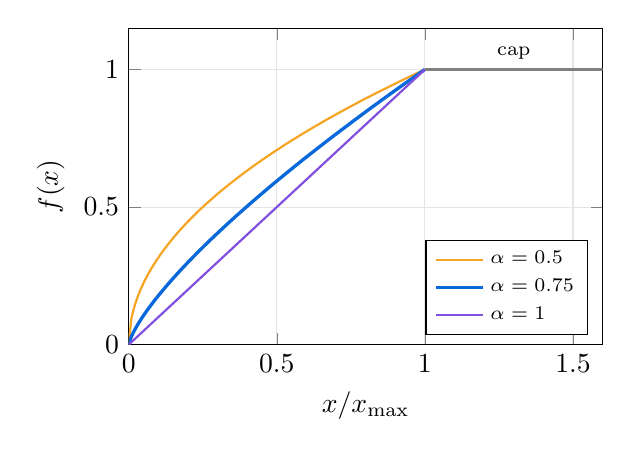
\begin{tikzpicture}
\begin{axis}[width=7.6cm,height=5.6cm,xlabel={$x/x_{\max}$},ylabel={$f(x)$},
  xmin=0,xmax=1.6,ymin=0,ymax=1.15,grid=major,grid style={gray!20},
  legend pos=south east,legend style={font=\scriptsize},legend cell align=left]
  \addplot[thick,wB,domain=0:1,samples=120]{x^0.5};
  \addplot[very thick,accent,domain=0:1,samples=120]{x^0.75};
  \addplot[thick,wE,domain=0:1,samples=60]{x};
  \addplot[very thick,gray,domain=1:1.6,forget plot]{1};
  \legend{$\alpha=0.5$,$\alpha=0.75$,$\alpha=1$}
  \node[font=\scriptsize,anchor=south] at (axis cs:1.3,1) {cap};
\end{axis}
\end{tikzpicture}
\end{columns}
\end{frame}

\begin{frame}{GloVe as weighted matrix factorisation}
\centering
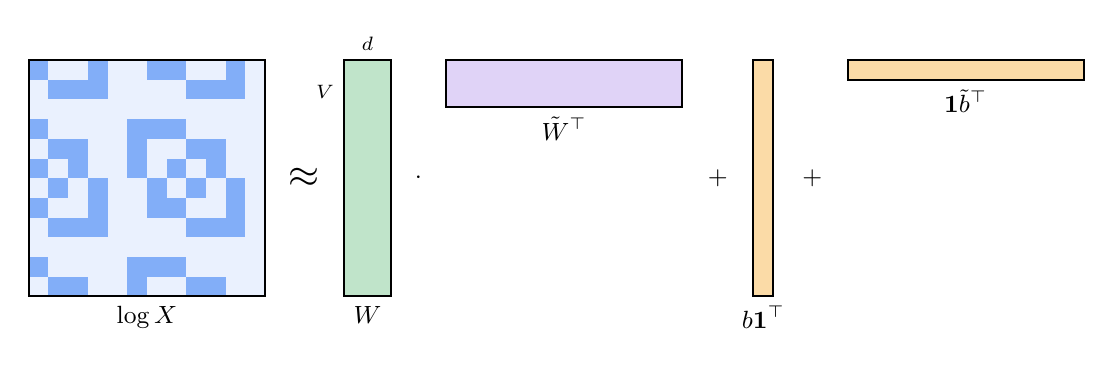
\begin{tikzpicture}[font=\small]
  \fill[wA!12] (0,0) rectangle (3,3);
  \foreach \i in {0,...,11} \foreach \j in {0,...,11} {
     \pgfmathsetmacro{\z}{mod(\i*\j+3*\i+5*\j,7)}
     \ifdim \z pt<3pt \fill[wA!70] (\j*0.25,3-\i*0.25-0.25) rectangle ++(0.25,0.25); \fi}
  \draw[thick] (0,0) rectangle (3,3);
  \node[below] at (1.5,0) {$\log X$};
  \node at (3.5,1.5) {\Large$\approx$};
  \fill[wC!30] (4,0) rectangle (4.6,3); \draw[thick] (4,0) rectangle (4.6,3);
  \node[below] at (4.3,0) {$W$}; \node[left,font=\scriptsize] at (4,2.6) {$V$}; \node[above,font=\scriptsize] at (4.3,3) {$d$};
  \node at (4.95,1.5) {$\cdot$};
  \fill[wE!25] (5.3,2.4) rectangle (8.3,3); \draw[thick] (5.3,2.4) rectangle (8.3,3);
  \node[below] at (6.8,2.4) {$\tilde W^{\top}$};
  \node at (8.75,1.5) {$+$};
  \fill[wB!40] (9.2,0) rectangle (9.45,3); \draw[thick] (9.2,0) rectangle (9.45,3);
  \node[below] at (9.33,0) {$b\mathbf 1^\top$};
  \node at (9.95,1.5) {$+$};
  \fill[wB!40] (10.4,2.75) rectangle (13.4,3); \draw[thick] (10.4,2.75) rectangle (13.4,3);
  \node[below] at (11.9,2.75) {$\mathbf 1\tilde b^{\top}$};
\end{tikzpicture}

\vspace{4mm}
\begin{itemize}\small
  \item A rank-$d$ approximation of $\log X$, plus row and column offsets.
  \item The loss is evaluated only on \textcolor{wA}{observed cells}, each weighted by $f(X_{ij})$, unlike SVD, which weights all cells equally.
  \item The problem is non-convex but well behaved, and is solved by stochastic gradient methods (AdaGrad, adaptive gradient, in the paper).
\end{itemize}
\end{frame}

\begin{frame}{Learning dynamics: what a gradient step does}
\footnotesize
\begin{columns}[c]
\column{0.5\textwidth}
Let $e_{ij}=\wv_i^\top\cv_j+b_i+\tilde b_j-\log X_{ij}$ (prediction error).
\begin{align*}
\nabla_{\wv_i}J&=2f(X_{ij})\,e_{ij}\,\cv_j\\
\nabla_{\cv_j}J&=2f(X_{ij})\,e_{ij}\,\wv_i\\
\partial_{b_i}J&=\partial_{\tilde b_j}J=2f(X_{ij})\,e_{ij}
\end{align*}
\small
\begin{itemize}
  \item $e<0$ (pair seen \emph{more} than predicted): pull $\wv_i$ and $\cv_j$ \alert{together}.
  \item $e>0$: push them apart.
  \item The step is scaled by $f$, so trusted (frequent) pairs move the vectors more.
\end{itemize}
\column{0.5\textwidth}
\centering
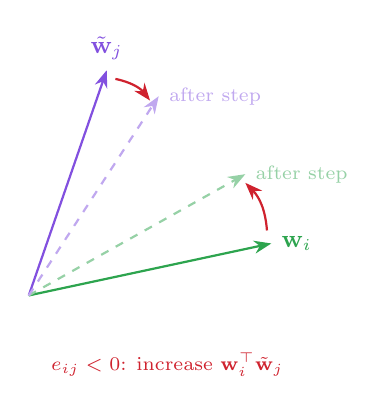
\begin{tikzpicture}[scale=1.1]
  \coordinate (o) at (0,0);
  \draw[arr,wC] (o) -- (2.8,0.6) node[right,font=\small]{$\wv_i$};
  \draw[arr,wE] (o) -- (0.9,2.6) node[above,font=\small]{$\cv_j$};
  \draw[arr,wC!50,dashed] (o) -- (2.5,1.4) node[right,font=\scriptsize]{after step};
  \draw[arr,wE!50,dashed] (o) -- (1.5,2.3) node[right,font=\scriptsize]{after step};
  \draw[arr,warn] (2.75,0.75) to[bend right=20] (2.5,1.3);
  \draw[arr,warn] (1.0,2.5) to[bend left=20] (1.4,2.25);
  \node[font=\scriptsize,warn,align=center] at (1.6,-0.8) {$e_{ij}<0$: increase $\wv_i^\top\cv_j$};
\end{tikzpicture}
\end{columns}
\end{frame}

\begin{frame}{Two vector sets, one embedding}
\small
\begin{columns}[c]
\column{0.55\textwidth}
\begin{itemize}\setlength\itemsep{1pt}
  \item The model learns $W$ (words) and $\tilde W$ (contexts).
  \item When $X$ is symmetric, $W$ and $\tilde W$ are \alert{equivalent}: they differ only because of random initialisation.
  \item The paper uses $\wv_i+\cv_i$ as the final representation:
    \begin{itemize}\small
      \item a cheap ensemble that reduces overfitting and noise;
      \item a small but consistent gain on analogy tasks.
    \end{itemize}
  \item Both vectors also enter similarity as $\wv_i^\top\cv_j+\ldots$, so the sum mixes first- and second-order similarity.
\end{itemize}
\column{0.45\textwidth}
\centering
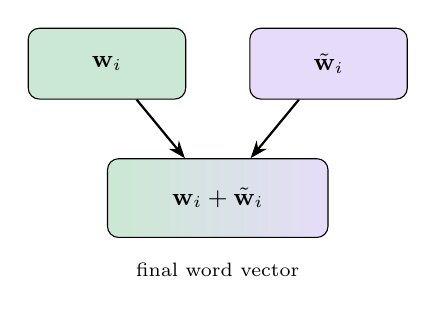
\begin{tikzpicture}[font=\small]
  \node[box,fill=wC!25,minimum width=20mm,minimum height=9mm] (w) {$\wv_i$};
  \node[box,fill=wE!20,minimum width=20mm,minimum height=9mm,right=8mm of w] (c) {$\cv_i$};
  \node[box,minimum width=28mm,minimum height=10mm,below=12mm of $(w)!0.5!(c)$,left color=wC!25,right color=wE!20] (s) {$\wv_i+\cv_i$};
  \draw[arr] (w) -- (s); \draw[arr] (c) -- (s);
  \node[font=\scriptsize,below=2mm of s] {final word vector};
\end{tikzpicture}
\end{columns}
\end{frame}

% =====================================================================
\section{Connections}
% =====================================================================

\begin{frame}{GloVe and pointwise mutual information}
\[
\PMI(i,j)=\log\frac{P(i,j)}{P(i)P(j)}=\log X_{ij}-\log X_i-\log X_j+\log|X|
\]
\begin{columns}[c]
\column{0.55\textwidth}
\small
Compare with GloVe's model:
\[
\wv_i^\top\cv_j=\log X_{ij}-b_i-\tilde b_j
\]
If the learned biases were $b_i=\log X_i$ and $\tilde b_j=\log X_j-\log|X|$, then
\[
\wv_i^\top\cv_j=\PMI(i,j).
\]
GloVe can be read as a \alert{weighted low-rank factorisation of a (shifted) PMI matrix}, where the shift is learned through the free biases instead of being fixed.
\column{0.45\textwidth}
\centering
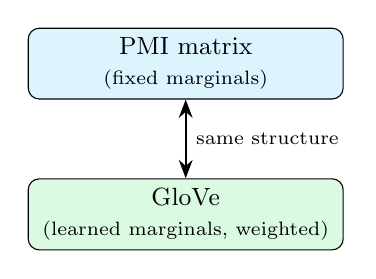
\begin{tikzpicture}[font=\small]
  \node[box,fill=stageA,minimum width=40mm] (pmi) {PMI matrix\\ \scriptsize (fixed marginals)};
  \node[box,fill=stageD,minimum width=40mm,below=10mm of pmi] (gl) {GloVe\\ \scriptsize (learned marginals, weighted)};
  \draw[arr,{Stealth}-{Stealth}] (pmi) -- node[right,font=\scriptsize]{same structure} (gl);
\end{tikzpicture}
\end{columns}
\end{frame}

\begin{frame}{GloVe and skip-gram (word2vec)}
\small
Skip-gram (SG) models $Q_{ij}=\dfrac{\exp(\wv_i^\top\cv_j)}{\sum_k\exp(\wv_i^\top\cv_k)}$. Summed over the corpus, its loss groups into
\[
J_{\text{SG}}=-\sum_{i,j}X_{ij}\log Q_{ij}=\sum_i X_i\,H(P_i,Q_i)
\]
a \emph{frequency-weighted cross-entropy} between the empirical $P_i$ and the model $Q_i$.
\vspace{2mm}
\begin{columns}[T]
\column{0.5\textwidth}
\textbf{Problems}
\begin{itemize}
  \item Normalising $Q$ costs $O(V)$ per term.
  \item Cross-entropy puts too much weight on unlikely events.
  \item The weight $X_i$ is unbounded.
\end{itemize}
\column{0.5\textwidth}
\textbf{GloVe's replacements}
\begin{itemize}
  \item Unnormalised $\hat P_{ij}=X_{ij}$ and $\hat Q_{ij}=\exp(\wv_i^\top\cv_j)$.
  \item Squared error on \alert{logs}: $(\log\hat Q-\log\hat P)^2$.
  \item The weight $X_i$ is replaced by the bounded $f(X_{ij})$.
\end{itemize}
\end{columns}
\vspace{2mm}
\centering\small The result is exactly the GloVe objective. The two methods use the same statistics with different losses.
\end{frame}

\begin{frame}{Where GloVe sits}
\small
\centering
\begin{tabular}{p{30mm}p{30mm}p{30mm}p{34mm}}
\toprule
 & \textbf{LSA / PPMI + SVD} & \textbf{skip-gram} & \textbf{GloVe}\\
\midrule
statistics & global counts & local windows & global counts\\
target & counts / PMI & next-context prob. & $\log X_{ij}$\\
loss & unweighted squared (SVD) & cross-entropy (sampled) & weighted squared\\
weighting & uniform over all cells & implicit $\propto X_i$ & explicit, capped $f(X_{ij})$\\
cost per epoch & one-off SVD & $O(|C|)$ & $O(\mathrm{nnz}(X))$\\
linear analogies & weak & strong & strong\\
\bottomrule
\end{tabular}

\vspace{5mm}
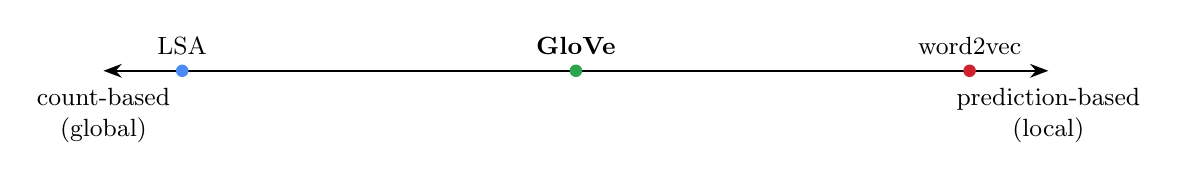
\begin{tikzpicture}[font=\small]
  \draw[thick,{Stealth}-{Stealth}] (0,0) -- (12,0);
  \node[below,align=center] at (0,-0.1) {count-based\\(global)};
  \node[below,align=center] at (12,-0.1) {prediction-based\\(local)};
  \node[pt,wA,label=above:{LSA}] at (1,0) {};
  \node[pt,wC,label=above:{\textbf{GloVe}}] at (6,0) {};
  \node[pt,wD,label=above:{word2vec}] at (11,0) {};
\end{tikzpicture}
\end{frame}

% =====================================================================
\section{Complexity}
% =====================================================================

\begin{frame}{How many non-zeros? A power-law argument}
\small
Model the co-occurrence counts as a power law in their frequency rank $r$: $X_{ij}=k/r_{ij}^{\,\alpha}$.\\
Since the corpus size is $|C|\propto\sum X_{ij}$, a generalised harmonic sum gives
\[
|C|\sim k\,\frac{|X|^{1-\alpha}}{1-\alpha}+k\,\zeta(\alpha)
\quad\Longrightarrow\quad
|X|=\begin{cases}O(|C|) & \alpha<1\\ O\big(|C|^{1/\alpha}\big) & \alpha>1\end{cases}
\]
\begin{columns}[c]
\column{0.5\textwidth}
\begin{itemize}
  \item The paper fits $\alpha\approx1.25$, so $|X|=O(|C|^{0.8})$.
  \item GloVe's cost per epoch is $O(|X|)$, which is \alert{sub-linear in corpus size}.
  \item Window-based methods scale as $O(|C|)$.
\end{itemize}
\column{0.5\textwidth}
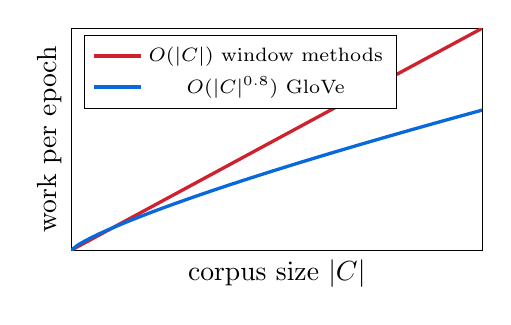
\begin{tikzpicture}
\begin{axis}[width=6.8cm,height=4.4cm,xlabel={corpus size $|C|$},ylabel={work per epoch},
  xmin=0,xmax=10,ymin=0,ymax=10,ticks=none,legend pos=north west,legend style={font=\scriptsize}]
  \addplot[very thick,wD,domain=0:10]{x};
  \addplot[very thick,accent,domain=0:10,samples=60]{x^0.8};
  \legend{$O(|C|)$ window methods,$O(|C|^{0.8})$ GloVe}
\end{axis}
\end{tikzpicture}
\end{columns}
\end{frame}

% =====================================================================
\section{Behaviour \& limitations}
% =====================================================================

\begin{frame}{Effect of the main choices (qualitative)}
\begin{columns}[c]
\column{0.5\textwidth}
\centering
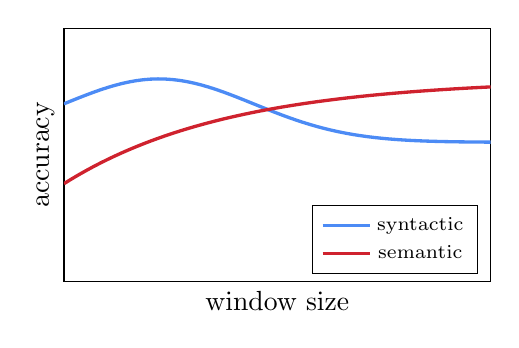
\begin{tikzpicture}
\begin{axis}[width=7cm,height=4.8cm,xlabel={window size},ylabel={accuracy},
  ticks=none,xmin=1,xmax=10,ymin=0,ymax=1,legend pos=south east,legend style={font=\scriptsize}]
  \addplot[very thick,wA,domain=1:10,samples=60]{0.55+0.25*exp(-(x-3)^2/8)};
  \addplot[very thick,wD,domain=1:10,samples=60]{0.25+0.55*(1-exp(-x/3.5))};
  \legend{syntactic,semantic}
\end{axis}
\end{tikzpicture}

{\scriptsize schematic, after Pennington et al.\ (2014), Fig.~2}
\column{0.5\textwidth}\small
\begin{itemize}
  \item \textbf{Window size}: small windows capture \emph{syntax} (local, word-order cues); large windows capture \emph{semantics} (topical association).
  \item \textbf{Dimension $d$}: gains flatten out around 200--300.
  \item \textbf{Corpus size}: more data steadily helps semantic tasks, and the corpus domain matters (encyclopaedic text helps factual analogies).
  \item \textbf{$x_{\max}$, $\alpha$}: fairly robust; $\alpha=\tfrac34$ beats $\alpha=1$.
\end{itemize}
\end{columns}
\end{frame}

\begin{frame}{Evaluating embeddings}
\begin{columns}[c]
\column{0.5\textwidth}
\centering
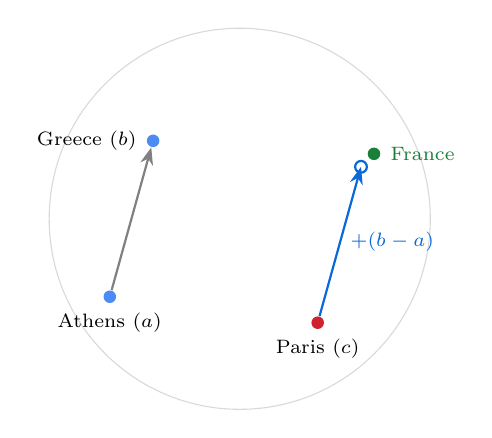
\begin{tikzpicture}[scale=1.1]
  \draw[gray!30] (0,0) circle (2.2);
  \node[pt,wA,label={[font=\scriptsize]below:Athens ($a$)}] (a) at (-1.5,-0.9) {};
  \node[pt,wA,label={[font=\scriptsize]left:Greece ($b$)}] (b) at (-1.0,0.9) {};
  \node[pt,wD,label={[font=\scriptsize]below:Paris ($c$)}] (c) at (0.9,-1.2) {};
  \coordinate (q) at (1.4,0.6);
  \node[pt,okc,label={[font=\scriptsize,okc]right:France}] at (1.55,0.75) {};
  \draw[arr,gray] (a) -- (b);
  \draw[arr,accent,thick] (c) -- node[right,font=\scriptsize]{$+(b-a)$} (q);
  \node[draw,accent,circle,inner sep=1.5pt,thick] at (q) {};
\end{tikzpicture}
\column{0.5\textwidth}\small
\textbf{Analogy} ($a:b::c:?$): pick the word closest in cosine to $\wv_b-\wv_a+\wv_c$, excluding $a,b,c$.
Split into semantic (capitals, family, \ldots) and syntactic (tense, plural, \ldots) questions.

\vspace{2mm}
\textbf{Similarity}: rank correlation between $\cos(\wv_i,\wv_j)$ and human ratings (WordSim-353, SimLex, \ldots).

\vspace{2mm}
\textbf{Downstream}: use the vectors as features, e.g.\ for named-entity recognition.
\end{columns}
\end{frame}

\begin{frame}{Limitations}
\begin{columns}[c]
\column{0.55\textwidth}
\begin{itemize}\small
  \item \textbf{One vector per word type}: senses are blended (\emph{bank}: river vs.\ finance).
  \item \textbf{Static}: the same vector in every sentence. Contextual models such as ELMo (Embeddings from Language Models) and BERT (Bidirectional Encoder Representations from Transformers) address this.
  \item \textbf{Closed vocabulary}: no vector for unseen words, and no subword information (unlike fastText).
  \item \textbf{Inherits corpus biases}, e.g.\ gender and occupation associations.
  \item \textbf{Symmetric context} loses word order beyond window distance.
\end{itemize}
\column{0.45\textwidth}
\centering
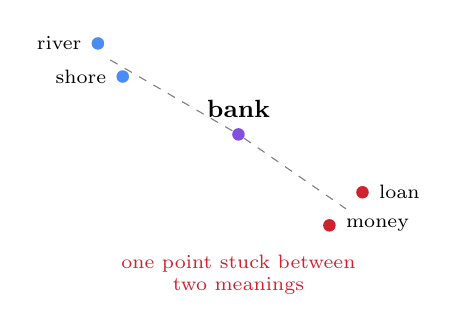
\begin{tikzpicture}[scale=1.05,lbl/.style={font=\scriptsize}]
  \node[pt,wA,label={[lbl]left:river}] at (0.2,2.4) {};
  \node[pt,wA,label={[lbl]left:shore}] at (0.5,2.0) {};
  \node[pt,wD,label={[lbl]right:loan}] at (3.4,0.6) {};
  \node[pt,wD,label={[lbl]right:money}] at (3.0,0.2) {};
  \node[pt,wE,minimum size=4pt,label={[font=\small\bfseries]above:bank}] (bk) at (1.9,1.3) {};
  \draw[dashed,gray] (0.35,2.2) -- (bk) -- (3.2,0.4);
  \node[font=\scriptsize,warn,align=center] at (1.9,-0.4) {one point stuck between\\two meanings};
\end{tikzpicture}
\end{columns}
\end{frame}

% =====================================================================
\section{Summary}
% =====================================================================

\begin{frame}{GloVe in one picture}
\centering
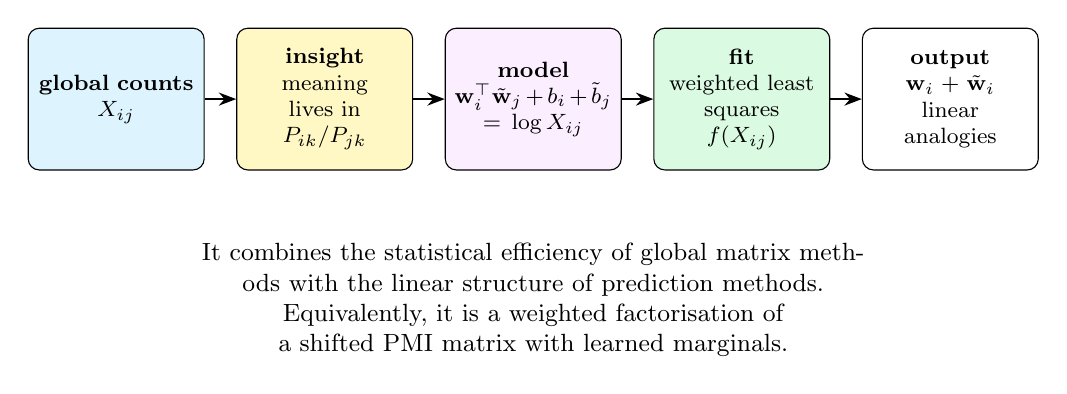
\begin{tikzpicture}[font=\small,node distance=4mm,
  s/.style={draw,rounded corners,align=center,minimum height=18mm,text width=20mm,font=\footnotesize}]
  \node[s,fill=stageA] (a) {\textbf{global counts}\\$X_{ij}$};
  \node[s,fill=stageB,right=of a] (b) {\textbf{insight}\\meaning lives in\\$P_{ik}/P_{jk}$};
  \node[s,fill=stageC,right=of b] (c) {\textbf{model}\\$\wv_i^\top\cv_j+b_i+\tilde b_j$\\$=\log X_{ij}$};
  \node[s,fill=stageD,right=of c] (d) {\textbf{fit}\\weighted least\\squares\\$f(X_{ij})$};
  \node[s,fill=white,right=of d] (e) {\textbf{output}\\$\wv_i+\cv_i$\\linear analogies};
  \foreach \x/\y in {a/b,b/c,c/d,d/e} \draw[arr] (\x) -- (\y);
  \node[below=8mm of c,text width=125mm,align=center]
   {It combines the \alert{statistical efficiency} of global matrix methods with the \alert{linear structure} of prediction methods.\\
    Equivalently, it is a weighted factorisation of a shifted PMI matrix with learned marginals.};
\end{tikzpicture}
\end{frame}

\begin{frame}{References}
\small
\begin{enumerate}
  \item J.~Pennington, R.~Socher, C.~D.~Manning. \emph{GloVe: Global Vectors for Word Representation}. Empirical Methods in Natural Language Processing (EMNLP) 2014.
  \item T.~Mikolov et al. \emph{Distributed Representations of Words and Phrases and their Compositionality}. Neural Information Processing Systems (NeurIPS) 2013.
  \item O.~Levy, Y.~Goldberg. \emph{Neural Word Embedding as Implicit Matrix Factorization}. NeurIPS 2014.
  \item S.~Deerwester et al. \emph{Indexing by Latent Semantic Analysis}. Journal of the American Society for Information Science (JASIS) 1990.
  \item J.~R.~Firth. \emph{A synopsis of linguistic theory 1930--1955}. 1957.
  \item J.~Duchi, E.~Hazan, Y.~Singer. \emph{Adaptive Subgradient Methods} (AdaGrad). Journal of Machine Learning Research (JMLR) 2011.
\end{enumerate}
\end{frame}

\end{document}
